\documentclass{article}

\usepackage{graphicx}
\usepackage{tikz}
\usepackage{tikzsymbols}
\usetikzlibrary{calc,patterns,shapes.geometric}
\pagestyle{empty}
\usepackage[margin=0pt]{geometry}
\geometry{papersize={14in,12in}}

\def\centerarc[#1](#2)(#3:#4:#5){\draw[#1] ($(#2)+({#5*cos(#3)},{#5*sin(#3)})$) arc (#3:#4:#5);}

\begin{document}
	\begin{figure}
		\centering
		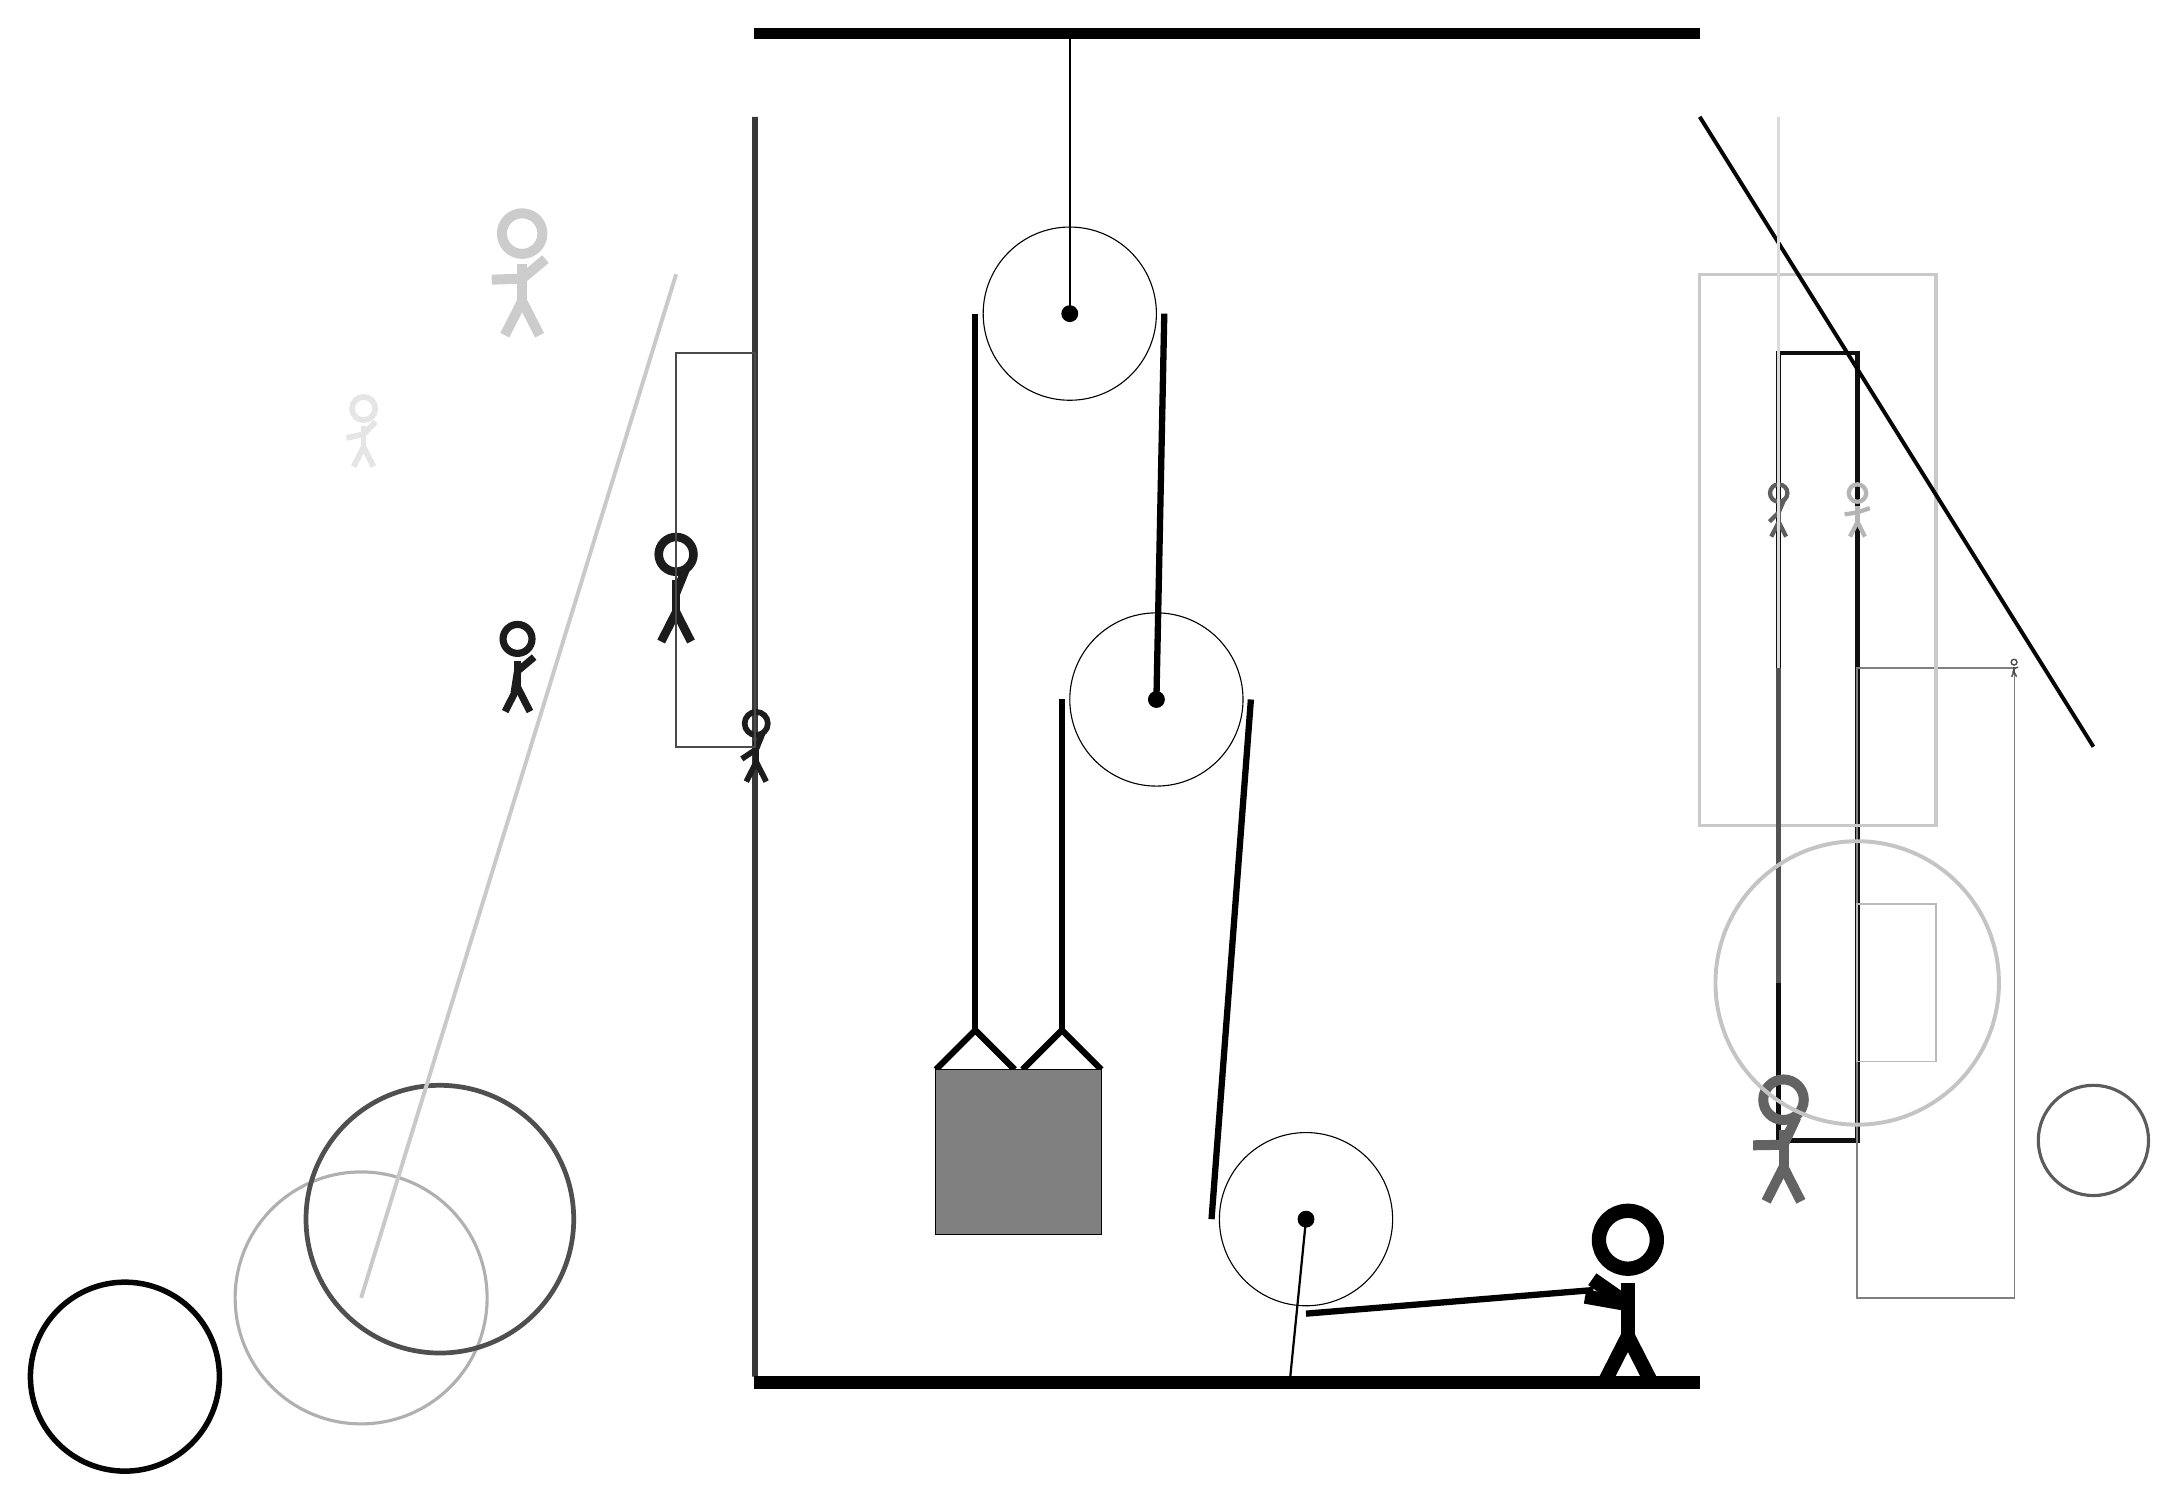
\begin{tikzpicture}
			%%%%% START %%%%%
			
			\draw[fill=black] (-2, 14) rectangle (10, 14.125);
			
			\draw[line width=0.6mm, color=black!46] (-4, 9) rectangle (-4, 9);
			
			\draw[line width=0.6mm, color=black!94] (11, 10) rectangle (12, 0);
			\draw[line width=0.2mm, color=black!50] (12, 6) rectangle (14, -2);
			\draw [line width=0.4mm, color=black!64](15, 0) circle (0.7);
			\node[line width=0.7mm, color=black!20] at (-5, 11) {\Strichmaxerl[7][2][40]};
			\draw [line width=0.4mm, color=black!31](-7, -2) circle (1.6);
			
			\draw[line width=0.4mm, color=black!21] (10, 4) rectangle (13, 11);
			\node[line width=0.5mm, color=black!10] at (-7, 9) {\Strichmaxerl[4][12][46]};
			\draw[line width=0.7mm, color=black!78] (-2, 13) rectangle (-2, -3);
			
			\draw [line width=0.6mm, color=black!69](-6, -1) circle (1.7);
			\node[line width=0.3mm, color=black!63] at (11, 8) {\Strichmaxerl[3][45][67]};
			
			\node[line width=0.2mm, color=black!89] at (-3, 7) {\Strichmaxerl[6][90][68]};
			\node[line width=0.6mm, color=black!89] at (-2, 5) {\Strichmaxerl[4][34][68]};
			\draw[line width=0.2mm, color=black!27] (12, 1) rectangle (13, 3);
			\draw [line width=0.7mm, color=black!98](-10, -3) circle (1.2);
			\node[line width=0.5mm, color=black!89] at (-5, 6) {\Strichmaxerl[5][81][40]};
			\node[line width=0.2mm, color=black!69] at (14, 6) {\Strichmaxerl[1][73][20]};
			\node[line width=0.3mm, color=black!29] at (12, 8) {\Strichmaxerl[3][9][19]};
			\node[line width=0.2mm, color=black!61] at (11, 0) {\Strichmaxerl[7][1][65]};
			\draw[line width=0.5mm, color=black!98](15, 5) -- (10, 13);
			\draw[line width=0.7mm, color=black!68] (11, 6) rectangle (11, 2);
			
			\draw[line width=0.3mm, color=black!71] (-2, 10) rectangle (-3, 5);
			\draw[line width=0.5mm, color=black!21](-7, -2) -- (-3, 11);
			\draw [line width=0.5mm, color=black!23](12, 2) circle (1.8);
			\draw[line width=0.4mm, color=black!14] (11, 13) rectangle (11, 6);
			
			
			\draw (2, 10.5) circle (1.1);
			\draw[fill=black] (2, 10.5) circle (0.1);
			\draw[thick] (2, 10.5) -- (2, 14);
			
			\draw (3.1, 5.6) circle (1.1);
			\draw[fill=black] (3.1, 5.6) circle (0.1);
			
			\draw (5, -1) circle (1.1);
			\draw[fill=black] (5, -1) circle (0.1);
			\draw[thick] (5, -1) -- (4.8, -3);
			
			\draw[line width = 0.8mm]  (0.3, 0.9) -- (0.8, 1.4) -- (1.3, 0.9);
			\draw[line width = 0.8mm]  (1.4, 0.9) -- (1.9, 1.4) -- (2.4, 0.9);
			\draw[fill=black!50] (0.3, 0.9) rectangle (2.4, -1.2);
			
			\draw[line width = 0.8mm] (0.8, 10.5) -- (0.8, 1.4);
			\centerarc[line width = 0.8mm](2, 10.5)(0:180:1.2000000000000002);
			\draw[line width = 0.8mm] (3.2, 10.5) -- (3.1, 5.6);
			\draw[line width = 0.8mm] (1.9, 5.6) -- (1.9, 1.4);
			\centerarc[line width = 0.8mm](3.1, 5.6)(0:180:1.2000000000000002);
			\draw[line width = 0.8mm] (4.3, 5.6) -- (3.8, -1);
			\centerarc[line width = 0.8mm](5, -1)(180:270:1.2000000000000002);
			\draw[line width = 0.8mm] (5, -2.2) -- (8.65, -1.9);
			
			\node at (9, -2) {\Strichmaxerl[10][-35][170]};
			
			\draw[fill=black] (-2, -3) rectangle (10, -3.15);
			
			%%%%% END %%%%%
		\end{tikzpicture}
	\end{figure}	
\end{document}